%========= Introduction
\section{Introduction}
\label{sec:introduction}

In the complex and ever-evolving world of \ac{EW}, quantum computing could provide the ability to understand radar signals in novel ways, never before seen in this field. 
It is widely recognised in the discipline of electronic warfare that traditional signal analysis techniques are still bounded by computational constraints, so in order to maintain strategic advantage, new techniques are continuously needed in order to keep pace with emerging threats. 
Quantum computing may promise a paradigmatic shift in extracting actionable insights from massive and complex \ac{EW} datasets. 

Recent research has demonstrated a great potential for quantum computing to address the challenges of modern signal processing \cite{somma_quantum_2019, daskin_walk_2022},
however little work has been devoted to its applications in \ac{EW} signal processing, and more specifically radar signal processing.
Therefore, this report explores the question of how quantum technology may be applied to radar signal processing in \ac{EW}.
At first, a survey of the current state of research will be conducted for radar signal analysis and quantum signal processing. 
\todojc{Perhaps this is where the last part of the "abstract" should merge with the following}Then, an empirical enquiry into the subject will be presented, aiming to determine how quantum methods can be used to encode, detect, and characterise radar signals.
Finally, a discussion of results, examination of limitations, and consideration for future work will be provided. 

Despite quantum computing holding much promise, its potential in this field remains largely unexplored.
This report presents a background and preliminary investigation into how quantum computing might be utilised in the dynamic landscape of electronic warfare. 

\subsection{Background}~\label{subsec:background}

%% Definition
\todojc{Perhaps a bit poetic for the scientific writing but nicely described}Much like the unrelenting noise of a bustling city street, the electromagnetic environment is chaotic and cacophonous.
Countless signals transmit through the air; under the radar of human perception, this deafening silence is critical to modern-day warfare.
With the electromagnetic spectrum being so chaotic and full of signals, it takes specialised tools and techniques to make sense of it all.
This is where \ac{ESM} plays a crucial role, enabling operators to gather valuable intelligence from the cacophonous electromagnetic environment.
Simply put, the goal is to use information from the spectrum to identify and locate potential threats.
Engineers and operators have developed advanced tools and techniques to overcome the challenges posed by this crowded environment, however the constraints of its inherent complexity and current technology still mean \ac{ESM} is an \todojc{Perhaps better to say "partially"}\textbf{unsolved problem}.

Among the countless signals that \ac{ESM} operators must sift through, radar signals are of particular interest due to their widespread use in military and civilian contexts.
Since radar's invention in 1930 \cite{degering_invention_2018}, it has been an invaluable tool for making the invisible visible.
\todojc{Best to avoid such colourful analogy in scientific writing, it would be good for magazine article one day, but not for thesis}\textbf{Like a blind person's white cane}, radar probes the environment to detect any potential impediments or hazards.
It is "an electrical system that transmits \ac{RF} electromagnetic waves toward a region of interest and receives and detects these EM waves when reflected from objects in that region."\cite{richards_principles_2010}.


% History

% Etymological
The name radar originates from a portmanteau of \textit{Radio Detection and Ranging}\cite{the_joint_board_on_scientific_information_policy_radar_1945}, hinting at it's founding objectives in the defence context. In the modern day, radar is used in many civilian and military applications \cite{merrill_i_skolnik_radar_nodate, desai_how_2022}:
\begin{itemize}
    \item Aerospace - weather, navigation, approach, altitude, identification
    \item Maritime - navigation, collision avoidance,  
    \item Ground Penetrating - archaeology, mining, oceanographic sounding
    \item Space - spacecraft and celestial monitoring
    \item Automotive - civilian and law enforcement
    \item Industrial - fluid sensing, speed measurement
    \item \todojc{some examples, as all above}Medical
    \item \todojc{some examples, as all above}Atmospheric / Weather
    \item \todojc{some examples, as all above}Electronic Warfare
\end{itemize}

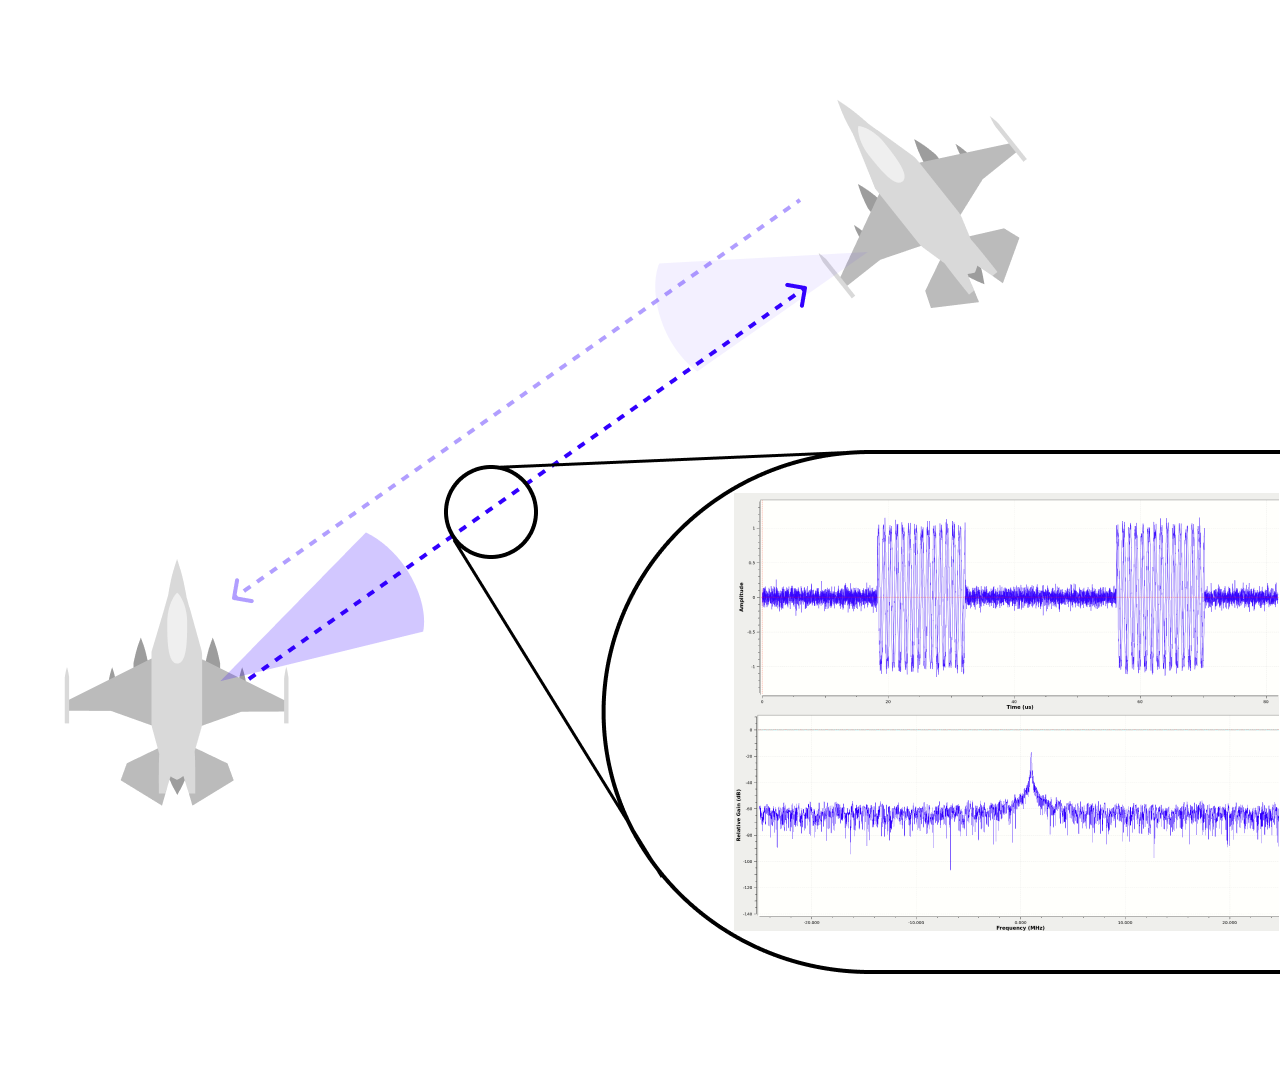
\includegraphics[width=\textwidth]{Figures/Senario_ Single Radar; single signal.png}
\todojc{All figures and tables need proper captions, which could be cross-referenced with text (with auto-numbering)}
% Consequence
As a result, the electromagnetic environment has become densely populated, with a multitude of different emitters posing a challenge of unintentional interference with operating radars \cite{degering_invention_2018}.
\todojc{This is very unclear, why multitude of emitters creating noise is a good thing}However, their widespread adoption - particularly in the defence context - yields the potential to identify the location and type of emitters in the area of operation.\todo{Passive; ESM}
This subject has been encompassed in the broader discipline of \ac{EW}. \ac{EW} is defined by David Adamy \cite{adamy_13_2001} as "the art and science of preserving the use of the electromagnetic spectrum for friendly use while denying its use to the enemy"\todo{I think a different definition would be best here, or perhaps referencing ELINT...}.

\ac{ESM}, a sub-field of \ac{EW}, where \ac{ESM} as "the receiving part of EW"\cite{adamy_13_2001}, of which radar is the principal element".

\todo{Describe the importance of radar \ac{ESM} here. Who cares and why? }


\todo{Principles of radar}

A typical radar system is made up of at least one of each: radio transmitter, radio receiver, antenna, and display \cite{stimson_introduction_1998}. % There was a more precise definition somewhere with a 'signal processor' element.

% The ESM pipeline
% ------------
% The sequence of radar processing:
% Pulse Detection:
% Target Association:
% Tracking:
% Classification:
% Decision:
% ------------------------------

\todo{Link back to:\ac{ESM} \ac{ECM} \ac{ECCM}. Here, consider providing a precise definition of \ac{ESM}. Also, somewhere here, a mention of \ac{ELINT} should be made}

For the radar to achieve its objectives, it must be able to convert observed data into actionable information, thereby requiring some degree of information processing. 
Herein lies the \todojc{Or are these really functions of ESM?}\textbf{general challenges} in \ac{ESM} - the detection, location, and identification of targets, which will now be explored. % Cite 'detection, location and identification' - I think the precise term is 'analysis'.

First, however, a conceptual schematisation of this system must be made in in terms of its inputs, process, and outputs. In \ac{ESM}, inputs consist of EM fluctuations that vary over time. They are almost always received by an antenna (or antennas) which may be subsequently manipulated in the analogue and digital domains. These fluctuations, henceforth \textit{signals} (not to be confused with communications signals), are the essential information carriers in the signal processing operation. There also exist inputs derived from the nature of the radar system configuration itself. These may include the antenna configuration and receiver architecture which will not here be considered, but is noted by the author as being of significant relevance to kinematic measurement and capability constraints.

Since the signals of interest are those emitted by radar systems, the received signals exhibit phenomenal qualities corresponding to those of the originating radar, namely: \todojc{Such a citation with page or section numbers are best written as \cite[sect. 5-8.1]{avionics_department_electronic_2013}}\cite{avionics_department_electronic_2013} 5-8.1\todojc{Would these parameters be best introduced as some chart annotations?}
\begin{itemize}
    \item Frequency (\ac{RF}): Intrapulse frequency, modulation (and associated modulation parameters); Interpulse: phase coherence.
    \item Amplitude (power)
    \item \ac{DOA} / \ac{AOA}
    \item \ac{TOA}
    \item \ac{PRI}, \ac{PRF}
    \item \ac{PRI} type
    \item \ac{PW}
    \item Scan type and rate
    \item Lobe duration (beam width or dwell)
\end{itemize}

The role of the processing step, is to convert the 'raw' signal into these parameters. Optimally, the parameters equal those nominally transmitted by the target radar.
These are generally extracted from the incident \ac{EM} signals and may be treated independently as outputs themselves. Typically, however, further analysis may be may conducted to yield very granular information. Information that \ac{ESM} seeks to understand addresses many facets:
\begin{itemize}
    \item \todojc{I assume "of targets"}Detection
    \item Target characteristics \cite{jenn_radar_2007}
    \begin{itemize}
        \item target size - return amplitude
        \item target shape - from discrete scan returns
        \item target material composition
        \item moving parts (modulation of the return)
    \end{itemize}
    \item Target identification
    \item Kinematic parameters and tracking(range, direction, speed, \ac{AOA})
\end{itemize}

\todo{Introduce multi-radar concept. - vignette}
\todo{Illustrate a scenario to make the problem more evident.}
\todojc{It is still unclear why we should go into a quantum solution, needs to better stage an argument, e.g. high complexity of problem / task / data, previous attempt with classical / AI / quantum solutions, need to look for better / more robust  solutions that are able to deal with x / y / z }
\todojc{\textbf{As I said this before, the background does not motivate the use of quantum tech, it does not even use the term "quantum" or "AI / ML", or why we'd need such clever solutions}}

\subsubsection{Research Question}
How can quantum computing methods be used to in an ESM function to detect the types and characteristics of radar signals in the defence context?

\subsubsection{Research Objectives}
\begin{itemize}
    \item Acquire a source data emulator to be used to test and verify quantum implementations.
    \item Identify the specific types of radar signals used in radar systems and their key signal parameters, based on an analysis of publicly available technical documents and datasets.
    \item Develop a quantum-based encoding method that converts sampled time-domain radar signals into qubits.
    \item Validate the quantum encoding method by evaluating the expressivity, complexity, and qualitative suitability.
    \item Develop a method for quantum-based pulse detection of a radar signals that vary in type and quality. The method must be quantifiably measurable.
    \item Validate the quantum pulse detection method by evaluating the accuracy of pulse boundary detection and signal-to-noise tolerance.
    \item Determine a quantum method for estimating a radar signal's frequency.
    \item Validate the frequency estimation method by evaluating the accuracy and signal-to-noise tolerance.
\end{itemize}

% Identify the challenge with multi-radar environments.

% Provide a brief outline of the genus of classical processing approaches.\
% Introduce quantum computing, and provide an abstracted overview of its potential application to this field.
% Conclude the case for quantum computing in ESM. Providce an implicit definition of the research question
% Identify the challenges with quantum computing.

% --------------
% OLD OBJECTIVES
% --------------
% In the processing functional block, the problems for radar are, in sequential order:
% \begin{itemize}
%     \item How to distinguish between the different categories of signals: communications, interference, radar, and noise.
%     \item Then, after having understood what signals are radar intercepts, identifying which belong to the same originating receiver. 
%     \item Once, a radar signal has been de-interleaved, how to identify the originating emitter, given some a priori understanding of the operational environment.
% \end{itemize}
% \begin{itemize}
%     \item To further understand the principles of operation of passive radar systems, including their ability to detect and identify emitters in complex electromagnetic environments.
%     \item To critically evaluate existing literature on radar systems and quantum computing to effecively communicate existing the academic knowledge, and to show a capability to conduct independent future research.
%     \item To identify the possibilities of using Quantum Computing in Radar signal analysis; to also identify three candidate avenues; to explore one in enough depth to evaluate potential feasability though the creation of a technical solution
%     \item To prioritize research topics based on their level of desirability and feasibility, and to develop a plan for executing research projects within a defined timeline and scope.
%     \item To communicate research findings effectively to a technical audience.
% \end{itemize}
% \begin{itemize}
%     \item Identify a candidate method, or methods for converting continuously varying parameterised radar signals into into discrete radar modes using quantum methods?
%     \item Is it possible, and to what extent are quantum methods effective in de-interleaving and signal clustering?
%     \item Can quantum computing effectively track a radar signal intercept, and how well?
%     \item %\almarginpar{Would the last two-four be in too hard basket for the time frame? May be better to leave those for the motivation section - if we could do the previous then we'd be able to do the following?}
%     In the radar context, can, and how well are quantum computing methods disposed to help in reducing noise, interference, and clutter?
% \end{itemize}
